% Document setup
\documentclass[12pt]{article}
\usepackage[margin=1in]{geometry}
\usepackage{fancyhdr}
\usepackage{lastpage}

\pagestyle{fancy}
\lhead{Richard Whitehill}
\chead{PHYS 804 -- HW \HWnum}
\rhead{\duedate}
\cfoot{\thepage \hspace{1pt} of \pageref{LastPage}}

% Encoding
\usepackage[utf8]{inputenc}
\usepackage[T1]{fontenc}

% Math/Physics Packages
\usepackage{amsmath}
\usepackage{amssymb}
\usepackage{mathtools}
\usepackage{physics}
\usepackage{siunitx}

\AtBeginDocument{\RenewCommandCopy\qty\SI}

% Enumeration/itemize
\usepackage{enumitem}
\newenvironment{parts}
{\begin{enumerate}[label=\textbf{(\alph*)},leftmargin=*,itemsep=-10pt]
}{\end{enumerate}}

% Reference Style
\usepackage{hyperref}
\hypersetup{
    colorlinks=true,
    linkcolor=blue,
    filecolor=magenta,
    urlcolor=cyan,
    citecolor=green
}

\newcommand{\eref}[1]{Eq.~(\ref{eq:#1})}
\newcommand{\erefs}[2]{Eqs.~(\ref{eq:#1})--(\ref{eq:#2})}

\newcommand{\fref}[1]{Fig.~\ref{fig:#1}}
\newcommand{\frefs}[2]{Figs.~\ref{fig:#1}--\ref{fig:#2}}

\newcommand{\tref}[1]{Table~\ref{tab:#1}}
\newcommand{\trefs}[2]{Tables~\ref{tab:#1}-\ref{tab:#2}}

% Figures and Tables 
\usepackage{graphicx}
\usepackage{float}
\usepackage[font=small,labelfont=bf]{caption}

\newcommand{\bef}{\begin{figure}[h!]\begin{center}}
\newcommand{\eef}{\end{center}\end{figure}}

\newcommand{\bet}{\begin{table}[h!]\begin{center}}
\newcommand{\eet}{\end{center}\end{table}}

% tikz
\usepackage{tikz}
\usetikzlibrary{calc}
\usetikzlibrary{decorations.pathmorphing}
\usetikzlibrary{decorations.markings}
\usetikzlibrary{arrows.meta}
\usetikzlibrary{positioning}
\usetikzlibrary{3d}
\usetikzlibrary{shapes.geometric}

% tcolorbox
\usepackage[most]{tcolorbox}
\usepackage{xcolor}
\usepackage{xifthen}
\usepackage{parskip}

\newcommand*{\eqbox}{\tcboxmath[
    enhanced,
    colback=black!10!white,
    colframe=black,
    sharp corners,
    size=fbox,
    boxsep=8pt,
    boxrule=1pt
]}

% problem-solution macros
% \usepackage{adjustbox}
\usepackage{changepage}

\newtcolorbox{probbox}[1][]{
    breakable,
    enhanced,
    boxrule=0pt,
    frame hidden,
    borderline west={4pt}{0pt}{green!50!black},
    colback=green!5,
    before upper=\textbf{Problem #1) \,},
    % \textbf{Problem #1 \ifthenelse{\isempty{#1}}{}{: #1} \\ },
    sharp corners,
    parbox=false
}

% \newtcolorbox{ProblemBox}[1][]{%
%   breakable,
%   enhanced,
%   colback=black!10!white,
%   colframe=black,
%   title={\large #1 \hfill}
% }
\newcommand{\prob}[2]{
\begin{probbox}[#1]
#2
\end{probbox}
}

\newenvironment{solution}{\begin{adjustwidth}{8pt}{8pt}}{\end{adjustwidth}}
\newcommand{\sol}[1]{
\begin{solution}
#1
\end{solution}
}
% \textbf{#1)} #2}

% Miscellaneous Definitions/Settings
\newcommand{\reals}{\mathbb{R}}
\newcommand{\integers}{\mathbb{Z}}
\newcommand{\naturals}{\mathbb{N}}
\newcommand{\rationals}{\mathbb{Q}}
\newcommand{\complexs}{\mathbb{C}}

\setlength{\parskip}{\baselineskip}
\setlength{\parindent}{0pt}
\setlength{\headheight}{14.49998pt}
\addtolength{\topmargin}{-2.49998pt}


\def\HWnum{Final Project}
\def\duedate{December 9, 2024}


\begin{document}

\begin{center}
    \textbf{\Large Numerical quantum scattering in one spatial dimension}
\end{center}

\section{Introduction}
\label{sec:introduction}

Scattering is one of the most productive methods used to date to learn about the structure and contents of our universe.
In a previous project this semester, we studied scattering from a central force field in a classical context by numerically integrating the ordinary differential equations of motion provided by Newton's $2^{\rm nd}$ law.
While Rutherford scattering is quite a robust problem, generating the same results in classical mechanics and Born level in quantum mechanics, realistically speaking, we should handle such systems quantum mechanically.
In this article, we make a first pass at studying scattering in a quantum mechanical regime, restricting our attention to only one dimension.

The remainder of this article is organized as follows.
In Sec. \ref{sec:mathematical-framework}, we set up the problem to be studied, remind ourselves of the analytic methods used to broach the problem, and finally detail the numerical techniques we will use to solve the problem numerically.
Next, in Sec. \ref{sec:numerical-simulations}, we apply our numerical schemes to some analytically solvable cases and discuss the performance of our numerical solutions.
Finally, in Sec. \ref{sec:conclusions}, we summarize our findings and remark on future work to improve them and extend toward a full three dimensional scattering framework.


\section{Mathematical framework}
\label{sec:mathematical-framework}


\subsection{Setting up the problem}

Our problem of interest in this article is one dimensional scattering in non-relativistic quantum mechanics.
As with all non-relativistic quantum mechanical problems, the fundamental equation governing all dynamics is the Schr\"{o}dinger equation\footnote{Note that we work in natural units where $\hbar = c = 1$. This implies that the time and spatial dimensions are equivalent as well as the energy, momentum, and mass dimensions. Additionally, in this system of units, the spatial and energy dimensions are inverses of each other, which allows us to remain agnostic regarding the exact scales of our problem.}
\begin{align}
\label{eq:td-S-eq}
    i \pdv{\Psi(x,t)}{t} = -\frac{1}{2m} \dv[2]{\Psi(x,t)}{x} + V(x) \Psi(x,t)
.\end{align}
The typical analytic method for solving these problems is to separate the temporal and spatial dependence as $\Psi_{E}(x,t) = e^{- i E t} \psi_{E}(x)$, where the stationary solution $\psi_{E}(x)$ satisfies the time-independent Schr\"{o}dinger equation with corresponding energy eigenvalue $E$:
\begin{align}
\label{eq:ti-S-eq}
    -\frac{1}{2m} \dv[2]{\psi_{E}}{x} + V(x) \psi_{E} = E \psi_{E}
.\end{align}
Because this is a Sturm-Liouville problem, the separable solutions are complete in our domain of interest, allowing us to expand any wave-function of interest in these separable solutions:
\begin{align}
\label{eq:psi-expansion}
    \Psi(x,t) = \sum_{E} c(E) e^{-i E t} \psi_{E}(x)
,\end{align}
where $|c(E)|^2$ denotes the relative contribution of a particular stationary state in the spectrum of our system to our wave function.
As a further remark, note that for this article, because we are interested in scattering, we will only include the so-called scattering states with $E > \lim_{|x| \rightarrow \infty} V(x)$ such that there is no contamination from bound states.
To this end, for the rest of our analytic treatment, we assume that our potential is localized such that $\lim_{|x| \rightarrow \infty} V(x) = 0$.
In this asymptotic region, we can treat our particle as free and describe it as a wave packet, constructd from plane waves $\psi_{k}(x) = e^{i k x}$ with $E = k^2 / 2m$.

\subsection{Wave packet treatment}
\label{ssec:wave-packet-treatment}

In order to understand the treatment of wave packets, we consider the case of a $\delta$-function potential given by $V(x) = V_0 \delta(x)$, which although not quite physical illustrates clearly the main ideas without much technical difficulty.
Clearly, the asymptotic regions are just $x < 0$ and $x > 0$, where our particle has momentum $\pm k$.
Although the eigenvalue $E = k^2/2m$ is doubly degenrate then, we choose the one corresponding to, as will become clear, an incident particle traveling from left to right and therefore $k > 0$ such that
\begin{align}
    \psi_{k}(x) = 
    \begin{cases}
        e^{i k x} + A(k) e^{-i k x} & x < 0 \\
        B(k) e^{i k x} & x > 0
    .\end{cases}
\end{align}
For our boundary conditions, we have $\psi_{k}(0^{-}) = \psi_{k}(0^{+})$ and $\psi_{k}'(0^{+}) - \psi_{k}'(0^{-}) = 2 m V_0 \psi_{k}'(0)$, which constrain our coefficients to be
\begin{align}
    A(k) &= -\frac{i V_0 m}{k + i V_0 m} \\
    B(k) &= \frac{k}{k + i V_0 m}
.\end{align}
We can then construct a wave-packet for all times $t$ by summing these energy eigenstates as follows:
\begin{align}
    \Psi(x,t) &= \int_{0}^{\infty} \frac{\dd{k}}{\sqrt{2 \pi}} g(k) \psi_{k}(x) \nonumber \\
              &= \Theta(-x) \Bigg\{ \int_{0}^{\infty} \frac{\dd{k}}{\sqrt{2 \pi}} g(k) e^{i k x - i k^2 t / (2m)} + \int_{0}^{\infty} \frac{\dd{k}}{\sqrt{2 \pi}} g(k) A(k) e^{-i k x - i k^2 t / (2m)} \Bigg\} \nonumber \\
              &+ \Theta(x) \int_{0}^{\infty} \frac{\dd{k}}{\sqrt{2 \pi}} g(k) B(k) e^{i k x - i k^2 t / (2m)}
,\end{align}
where $g(k)$ is some properly chosen real profile function.

We are now interested in understanding how the wave packet will appear after scattering from the potential.
The analysis is made more tractable and cleaner if our wave packets have momentum modes sharply centered at some $k = k_0$.
Making this assumption, we proceed via the method of stationary phase.
Let us analyze the form of each term separately, beginning with the incident wave packet
\begin{align}
    \Psi_{I}(x,t) = \int_{0}^{\infty} \frac{\dd{k}}{\sqrt{2 \pi}} g(k) e^{i \varphi_{I}(x,t,k)}
,\end{align}
where $\varphi_{I}(x,t,k) = kx - k^2 t / 2m$.
Since $g(k)$ is sharply peaked around some $k_0$, we expand the phase function about $k_{0}$ as
\begin{align}
    \varphi_{I}(x,t,k) &= \varphi_{I}(x,t,k_0) + (k - k_0) \dv{\varphi_{I}}{x}\Big|_{k=k_0} + \mathcal{O}\Big( (k - k_0)^2 \Big) \nonumber \\
                       &\approx \varphi_{I}(x,t,k_0) + (k - k_0) (x - x_{i}(t))
,\end{align}
where $x_{I}(t) = k_0 t / m$ satisfies $\dv*{\varphi_{I}}{k}|_{k=k_0,x=x_{I}(t)} = 0$ and is representative of the center of our incoming wave packet and corresponds approximately to the position of our wave packet with stationary phase, which is the inspiration for the method's name.
Using this, we write
\begin{align}
    \Psi_{I}(x,t) \approx e^{i \varphi_{I}(x,t,k_{0})} \int_{0}^{\infty} \frac{\dd{k}}{\sqrt{2 \pi}} g(k) e^{i (k - k_0) (x - x_{I}(t))}
.\end{align}
Observe that since $g(k)$ is sharply peaked around $k = k_0 > 0$, it is inconsequential to extend the integration range to all $k$ as
\begin{align}
    \Psi_{I}(x,t) &\approx e^{i \varphi_{I}(x,t,k_0)} \int_{-\infty}^{\infty} \frac{\dd{k}}{\sqrt{2 \pi}} g(k) e^{i (k - k_0) (x - x_{I}(t))} \nonumber \\
                  &= e^{i [ \varphi_{I}(x,t,k_0) - k_0 (x - x_{I}(t)) ]} \int \frac{\dd{k}}{\sqrt{2 \pi}} g(k) e^{i k ( x - x_{I}(t) )} \nonumber \\
                  &= e^{i[\varphi_{I}(x,t,k_0) - k_0 (x - x_{I}(t))]} G(x - x_{I}(t))
,\end{align}
where $G(x)$ is the inverse Fourier transform of $g(k)$.
Next, we analyze the form of the reflected wave packet.
Defining $A(k) = |A(k)| e^{-i \chi_{A}(k)}$ such that
\begin{align}
    |A(k)| = \frac{V_0^2 m^2}{k^2 + V_0^2 m^2}~{\rm and}~\tan{\chi_{A}(k)} = -\frac{k}{m V_0}
,\end{align}
we write
\begin{align}
    \Psi_{R}(x,t) = \int_{0}^{\infty} \frac{\dd{k}}{\sqrt{2 \pi}} g(k) |A(k)| e^{-i \varphi_{R}(k)}
,\end{align}
so that the overall reflected phase function
\begin{align}
    \varphi_{R}(x,t,k) = kx + \frac{k^2 t}{2m} + \chi_{A}(k)
.\end{align}
Performing the stationary phase expansion, we find
\begin{align}
    \varphi_{R}(x,t,k) \approx \varphi_{R}(x,t,k_0) + (k - k_0) (x - x_{R}(t))
,\end{align}
where 
\begin{align}
    x_{R}(t) &= - \frac{k_0 t}{m} - \chi_{r}'(k_0) = -\frac{k_0 t}{m} + \frac{1}{m V_0} \frac{1}{1 + {\rm arctan}^2(k_0 / m V_0)} \nonumber \\
    &= -\frac{k_0}{m} \Bigg\{ t - \frac{1}{k_0 V_0} \frac{1}{1 + \arctan^2(k_0/m V_0)} \Bigg\}
.\end{align}
With this, we have
\begin{align}
    \Psi_{R}(x,t) = |A(k_0)| e^{i [ \varphi_{R}(x,t,k_0) - k_0(x - x_{R}(t)) ]} G(x - x_{R}(t))
.\end{align}
Similarly, for the transmitted wave packet
\begin{align}
    \Psi_{T}(x,t) &= \int_{0}^{\infty} \frac{\dd{k}}{\sqrt{2 \pi}} g(k) |B(k)| e^{i \varphi_{T}(x,t,k)}
\end{align}
with $\varphi_{T}(x,t,k) = k x - k^2 t / (2m) - \chi_{B}(k)$ so that
\begin{align}
    x_{T}(t) = \frac{k_0 t}{m} + \chi_{B}'(k) = \frac{k_0}{m} \Bigg\{ t - \frac{m^2 V_0}{k_0^3} \frac{1}{1 + \arctan^2(m V_0 / k_0)} \Bigg\}
\end{align}
and
\begin{align}
    \Psi_{T}(x,t) = |B(k_0)| e^{i [ \varphi_{T}(x,t,k_0) - k_0 ( x - x_{T}(t) ) ]} G(x - x_{T}(t))
.\end{align}
With this, we have essentially concluded our analysis for scattering from a $\delta$-function potential with a wave packet moving with a nearly uniform momentum.

The upshot of all this work is the following.
When we prepare a wave packet with a very narrow momentum spectrum that is sent towards a localized momentum, then after a sufficient amount of time -- determined by the particle's mass and average momentum as well as the specifics of the potential -- we observe reflected and transmitted wave packets in the asymptotic region with approximately the same shape as our incident wave packet, modulated by some transmission and reflection amplitudes that obey probability conservation as
\begin{align}
    |A(k_0)|^2 + |B(k_0)|^2 = 1
,\end{align}
which can be shown by considering the normalization of the wave function in the asymptotic limits $t \rightarrow \pm \infty$.
Thus, $|A(k)|^2$ gives us the probability for a wave packet with momentum $k$ to scatter backwards toward $x \rightarrow -\infty$ while $|B(k)|^2$ gives us the probability for a wave packet to be transmitted through the potential and propagate toward $x \rightarrow \infty$.

In this article, our goal will be to map out the these reflection and transmission probabilities.
To this end, for our numerical simulations, we will prepare wave packet states localized in momentum space far from some potential of interest, evolve our system in time until we have our reflected and transmitted wave packets in the asymptotic region, and finally compute the reflection and transmission probabilities as
\begin{align}
\begin{aligned} 
    |A(k)|^2 &= \lim_{t \rightarrow \infty} \int \dd{x} |\Psi_{R}(x,t)|^2 \\
    |B(k)|^2 &= \lim_{t \rightarrow \infty} \int \dd{x} |\Psi_{T}(x,t)|^2
.\end{aligned}
\end{align}


\subsection{Numerical techniques for unitary time evolution}
\label{ssec:numerical-techniques-for-unitary-time-evolution}

According to Eq. (\ref{eq:psi-expansion}), if we know the spectrum of our theory, then we can automatically expand our wave packet in the scattering states with the time evolution given by the factor $e^{-i E t}$.
In practice, though, it may not be such a simple matter or even possible to solve the time-independent Schr\"{o}dinger equation for a given potential in closed form.
We could perhaps adopt the same approach as in Project 3 where we discretized Eq. (\ref{eq:ti-S-eq}) to transform it into an eigenvalue problem.
However, unlike in the case where we were interested in solving for bound state wave functions and energies, in the case of scattering states, we know \textit{a priori} our energy eigenvalues for scattering states and further that our energy spectrum is continuous.
Therefore, it is somewhat problematic to only receive a finite number of energy eigenvalues which we cannot necessarily gurantee will be centered on any momentum mode or how densely the eigenvalues would be spaced.
Additionally, for bound states, it is natural to impose Dirichlet conditions since our solutions must vanish in the asymptotic regions, but for the localized potentials here, our solutions will be plane waves.
Although, our physical wave packet must vanish far from the center, the separable solutions do not.

Because of the difficulties layed out above, instead of solving the time-independent Schr\"{o}dinger equation and splicing together the stationary states as in Eq. (\ref{eq:psi-expansion}), we will solve the time-dependent Schr\"{o}dinger equation directly with the boundary condition at $t = 0$ given by an appropriate wave packet.
The first attempt made to simulate the time evolution of a wave packet utilized the finite difference method, discretizing our spatial and temporal domain to yield a transfer matrix $U$ which evolved our wave function from one time slice to the next.
However, in practice, we do not use this method for a few troublesome reasons.
Primarily, though, the transfer matrix $U$ violates unitarity at the order of $\Delta t^2$, where $\Delta t$ is the size of the time step, and while this is not an issue over only a few time steps, the errors propagate dramatically over a sizable number of steps, which implies that probability is not properly conserved.
For more details on this method, a derivation and discussion are placed in App. \ref{app:finite-differences}.

Finally, we come to the Fourier transform inspired method that we use in our simulations.
Instead of discretizing our wave packets from the onset and obtaining a finite transfer matrix $U$, we recall that we can introduce the unitary time evolution operator $U(t,t')$, which evolves our wave function at time $t'$ to time $t$ via $\Psi(x,t) = U(t,t') \Psi(x,t')$.
From this requirement, we deduce that $U$ satisfies the operator equation
\begin{align}
    i \pdv{U(t,t')}{t} = H U(t,t')
,\end{align}
which has solution
\begin{align}
    U(t,t') = e^{-i H (t - t')}
\end{align}
if $H$ is independent of time as will be the case in our scattering problems.
Let us write $H = H_0 + V$, where $H_0$ is the free-particle Hamiltonian and $V$ contains the potential terms.
If we choose our time step $\Delta t$ between time slices $t_{m}$ and $t_{m+1}$ to be small, then using the Baker-Campbell-Hausdorff formula, we can write
\begin{align}
    U(\Delta t) &= e^{-i H \Delta t} = e^{-i H_0 \Delta t - i V \Delta t} \approx e^{-i H_0 \Delta t} e^{-i V \Delta t} e^{\frac{\Delta t^2}{2} [H_0, V]} \nonumber \\
                &= e^{-i H_0 \Delta t} e^{-i V \Delta t} \Big( 1 + \frac{\Delta t^2}{2} [H_0,V] + \mathcal{O}(\Delta t^{4}) \Big)
.\end{align}
For sufficiently small time steps, the free particle and potential pieces of the Hamiltonian can act separately on our wave packet, and because plane waves are eigenstates of the free particle Hamiltonian, we can express our wave function at the current time step $t_{m}$ as a Fourier transform and act the time evolution operator as follows:
\begin{align}
    \Psi(x,t_{m+1}) &= U(\Delta t) \Psi(x,t_{m}) = e^{-i V(x) \Delta t} \int \frac{\dd{k}}{\sqrt{2 \pi}} \widetilde{\Psi}(k,t_{m}) e^{-i H_0 \Delta t} e^{i k x} \nonumber \\
    &= e^{-i V(x) \Delta t} \int \frac{\dd{k}}{\sqrt{2 \pi}} \widetilde{\Psi}(k,t_{m}) e^{- i k^2 \Delta t / (2m)} e^{i k x}
,\end{align}
where $\widetilde{\Psi}(k,t_{m})$ is the Fourier transform of $\Psi(x,t_{m})$.
Thus, for small time steps our potential changes the phase of the wave-function locally while the free part of the Hamiltonian propagates our modes according to the velocity $k/m$.

Because the above equation is set up on the continuous spatial domain we could set up our wave-packets as functions numerically and implement a numerical quadrature to take the Fourier transform at each $x$, but this could become quite computationally expensive both regarding resources and time.
We could, however, discretize our spatial domain and use the discrete Fourier transform (DFT), computed via the fast-fourier transform method.

We note that in practice, we cannot simply replace the continuous Fourier transform (CFT) with a DFT and evaluate at the spatial grid points: we must include a few factors to correctly obtain the CFT from the DFT.
For brevity, consider some square integrable function $f(x)$.
The expressions we use for the continuous fourier and inverse fourier transforms of $f(x)$ are as follows:
\begin{align}
\begin{aligned} 
    f(x) &= \int \frac{\dd{k}}{\sqrt{2 \pi}} \tilde{f}(k) e^{i k x} \\
    \tilde{f}(k) &= \int \frac{\dd{x}}{\sqrt{2 \pi}} f(x) e^{-ikx}
.\end{aligned}
\end{align}
On the other hand, for a collection of discrete data points $f_{n}$, their discrete Fourier and inverse Fourier transforms are as follows (consistent with the \textit{numpy} conventions using the ``ortho'' normalization):
\begin{align}
\begin{aligned} 
    f_{n} &= \frac{1}{\sqrt{N}} \sum_{m=0}^{N-1} F_{m} e^{2 \pi i \frac{m n}{N}} \\
    F_{m} &= \frac{1}{\sqrt{N}} \sum_{n=0}^{N-1} f_{n} e^{-2 \pi i \frac{m n}{N}}
.\end{aligned}
\end{align}
We can write the grid points in $x$-space as $x_{n} = x_0 + n \Delta x$ and those in $k$-space as $k_{m} = m \Delta k$ with $n,m \in \{ 0,1,\ldots,N-1 \}$, where
\begin{align}
    \Delta x \Delta k = \frac{2 \pi}{N}
.\end{align}
From this discretization, we can approximate
\begin{align}
    \tilde{f}(k) = \sum_{n=0}^{N-1} \frac{\Delta x}{\sqrt{2 \pi}} f(x_{n}) e^{-i k x_{n}} = \frac{\Delta x \sqrt{N}}{\sqrt{2 \pi}} e^{-i k x_0} \frac{1}{\sqrt{N}} \sum_{n=0}^{N-1} f(x_{n}) e^{-i k n \Delta x}
.\end{align}
Hence,
\begin{align}
    \tilde{f}(k_{m}) = \frac{\Delta x \sqrt{N}}{\sqrt{2 \pi}} e^{-i k_{m} x_0} F_{m}
.\end{align}
We can also then perform the inverse fourier transform by writing $F_{m}$ in terms of $\tilde{f}(k_{m})$.

One thing to note with this method is that we have not imposed boundary conditions explicitly, but it can be seen that the Fourier method implicitly imposes periodic boundary conditions.
That is, any part of the wave packet which exits our physical numerical domain to the right appears back on the left part of our spatial domain and \textit{vice versa}.
To deal with this, we should ensure that our numerical domain is much larger than the extent of our potential such that our wave packets reach the asymptotic region before a significant portion of the transmitted or reflected wave packets enter the incorrect region of space and contribute to the wrong probability density.


\section{Numerical simulations}
\label{sec:numerical-simulations}

\subsection{Freely propagating Gaussian wave packet}
\label{ssec:freely-propagating-gaussian-wave-packet}

To test that our numerical solver works, we choose an initial wave function
\begin{align}
    \Psi(x,0) = \frac{1}{(2 \pi \sigma^2)^{1/4}} \exp{-\frac{(x - x_{0})^2}{4 \sigma^2}} \exp{i k x}
,\end{align}
which is a Gaussian density at $t = 0$ with average momentum $k$.
We can now use the propagator formalism to determine the wave function at any later time $t$ as $\Psi(x,t) = \int \dd{x'} K(x,x';t) \Psi(x',0)$, where for a free particle $K(x,x';t) = \sqrt{m/(2 \pi i t)} \exp{-m(x - x')^2/(2it)}$.
While the intermediate form of the wave function is not too interesting for our purposes, the probability density
\begin{align}
    |\Psi(x,t)|^2 = \frac{1}{\sqrt{2 \pi \sigma^2}} \frac{2 \sigma^2 m}{\sqrt{ 4 \sigma^4 m^2 + t^2 }} \exp{ -\frac{2 m^2 \sigma^2 [ x - (x_0 + k t / m) ]^2}{4 \sigma^{4} m^2 + t^2} }
.\end{align}
As a testing ground for our time evolution scheme, we plot the probability density at a few time slices as computed from the exact equation above and from a numerical simulation, starting from the wave packet provided at $t = 0$.
We can see qualitatively that the numerical and exact wave packets agree quite well, and indeed probability is conserved over a large time interval as needed.


\begin{figure}[tb]
    \centering
    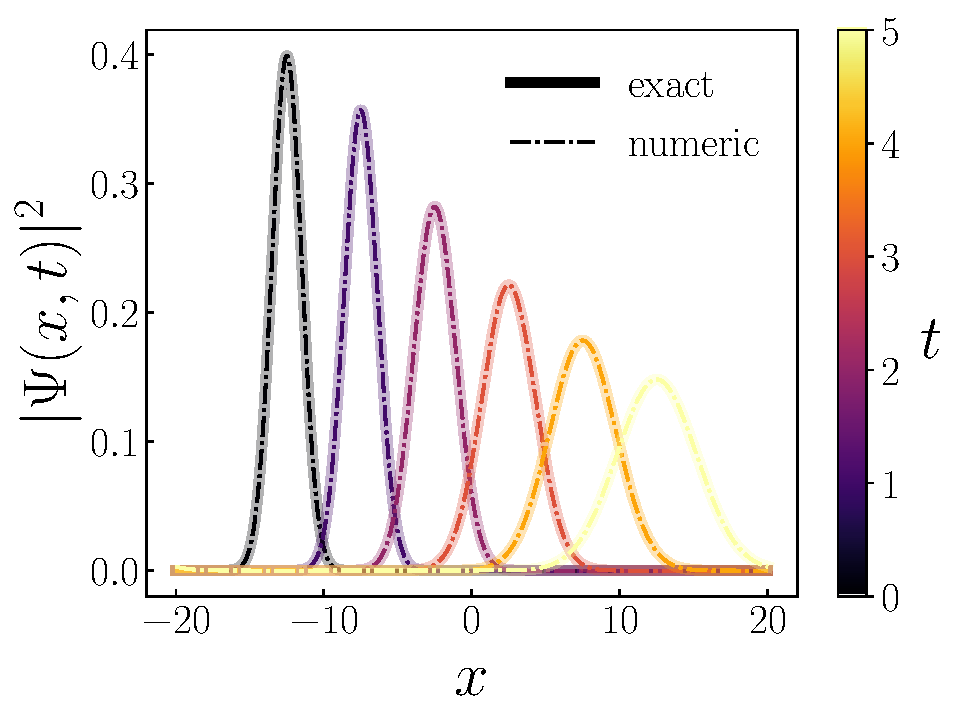
\includegraphics[width=0.7\linewidth]{gauss_wave-prop.pdf}
    \caption{Comparison of a particle with mass $m = 10$, propagating as a Gaussian wave packet with $k = 5$ and $\sigma = 1$, with the numerical Fourier transform based numerical scheme presented in Sec. \ref{ssec:numerical-techniques-for-unitary-time-evolution}.}
    \label{fig:gauss-wave-prop}
\end{figure}

While our time evolution is satisfactory for a free particle, before moving on to some examples of one-dimensional scattering, we examine more quantitatively what we mean by a sharply peaked wave packet.
In our treatment of wave packets, we assumed our wave packets were sharply, peaked in momentum space, enough such that they propagated without dispersing significantly.
From the form of the probability density above, we can see that this is indeed the case if
\begin{align}
    \frac{\sigma_{t}}{\sigma} = \sqrt{1 + \frac{t^2}{4 \sigma^{4} m^2}}
,\end{align}
where $\sigma_{t}$ represents the spread of our wave packet at time $t$.
Hence, if we simulate for a time $T$ before reaching asymptotic final states, then we should have $T^2 / 4 \sigma^{4} m^2 \ll 1$.
\textit{A priori}, though, we do not know for how long we should simulate.
Thus, if we place our incident wave packet at $x_{I}(t = 0) = x_0$ and expect roughly that the total time $T \approx 2 x_0 m / k$, then we should have $x_0^2 / \sigma^{4} k^2 \ll 1$.
A natural length scale is the initial spread of the wave packet $\sigma$, so if we further define $x_0 = M_2 \sigma$, we obtain
\begin{align}
    \sigma \gg \frac{M_2}{k}
.\end{align}
Thus, we can select some $M_1$ such that $\sigma = M_1 M_2 / k$ and the equation above is satisfied to some tolerance.
As another consideration, we must place our wave packet far away from the potential at $t = 0$.
But how far is far?
If our potential is centered at the origin and has some extent $a$, then we should select $M_2$ as defined above such that the probability of finding our particle at $t = 0$ in the region $x > -a/2$ is negligibly small, or practically speaking below some tolerance.

\subsection{Square barrier}
\label{ssec:square-barrier}

For this section, we consider a potential of the form $V(x) = V_0 [ \Theta(x) - \Theta(x - a) ]$.
We then find the following analytic expression for the transmission probability
\begin{align}
\label{eq:square-barrier-Pt}
    |B(k)|^2 = 
    \begin{cases}
        \dfrac{4 \kappa^2 k^2}{4 \kappa^2 k^2 + 4 m^2 V_0^2 \sinh^2(\kappa a)} & k < \sqrt{2 m V_0} \\
        \dfrac{k^2 a^2}{k^2 a^2 + 4} & k = \sqrt{2 m V_0} \\
        \dfrac{4 k'^2 k^2}{4 k'^2 k^2 + 4 m^2 V_0^2 \sin^2(k' a)} & k > \sqrt{2 m V_0}
    ,\end{cases}
\end{align}
where $\kappa^2 = 2 m V_0 - k^2$ and $k' = k^2 - 2 m V_0$.
In Fig. \ref{fig:square-barrier}, we plot the results of a numerical simulation for this scattering process on top of the exact analytic result for some selected $V_0$, $a$, and $m$.
We note that our range in $k$ goes up to $m$, which calls into question whether our example indeed is governed by non-relativistic quantum mechanics.
However, technically speaking, there is no kinematic restriction placed on the values of $k$ by the theory, so for practical purposes we have allowed $k$ to range up to such not quite physical values in order to assess the quality of our simulations without resorting to lengthy calculations, and indeed, we note a relatively good agreement once we reach larger values of $k$.

We remark, though, that as for a typical lattice simulation, we require a significant amount time and computational resources to obtain accurate results\footnote{In order to produce Fig. \ref{fig:square-barrier}, it took 20.5 minutes with four jobs running in parallel at a time.}, and furthermore, there are a number of parameters presented here that can be fine-tuned in order to obtain more accurate results.
A first general source of error and computational load is the size of our time step.
By design our method is more accurate when $\Delta t \rightarrow 0$, and it is increasingly important to reduce our time step when $k/m$ is larger so that we do not have our wave packet propagate through our potential without interacting.
Another source of errors stems from the discrete Fourier transform, although these are slightly more subtle and less explored in this article.
Lastly, our initial configuration contributes significantly to the computational load required to complete a scattering simulation at a given $k$.
For example, for smaller $k/m$, as discussed in Sec. \ref{ssec:freely-propagating-gaussian-wave-packet}, we require a larger spread in our initial wave packet, which in turn requires us to keep a larger spatial domain on which to simulate.
Naively, we should also expect to increase the number of points in our spatial domain when $\sigma$ increases, but this may not quite be the case.
Recall that the grid spacing in coordinate and momentum space are related as $\Delta x \Delta k = 2 \pi / N$.
ALthough not done here, we leave for a future work a more extensive study toward understanding how to select $\Delta x$ and $\Delta k$ which are both small enough.
Of course, in coordinate space, we require $\Delta x$ to be small enough so that our computation of the reflection and transmission probabilities using basic rectangular Riemann sums do not degrade, although this can be improved by using better numerical quadrature techniques as well.
Meanwhile, we also must ensure that $\Delta k$ is small enough since we design our wave packets such that their Fourier transforms are sharply peaked around a particular momentum.
Hence, the support on the momentum domain is very narrow, and if $\Delta k$ is not small enough, after evolving in time, we can miss important contributions to the inverse discrete Fourier transform.

\begin{figure}[tb]
    \centering
    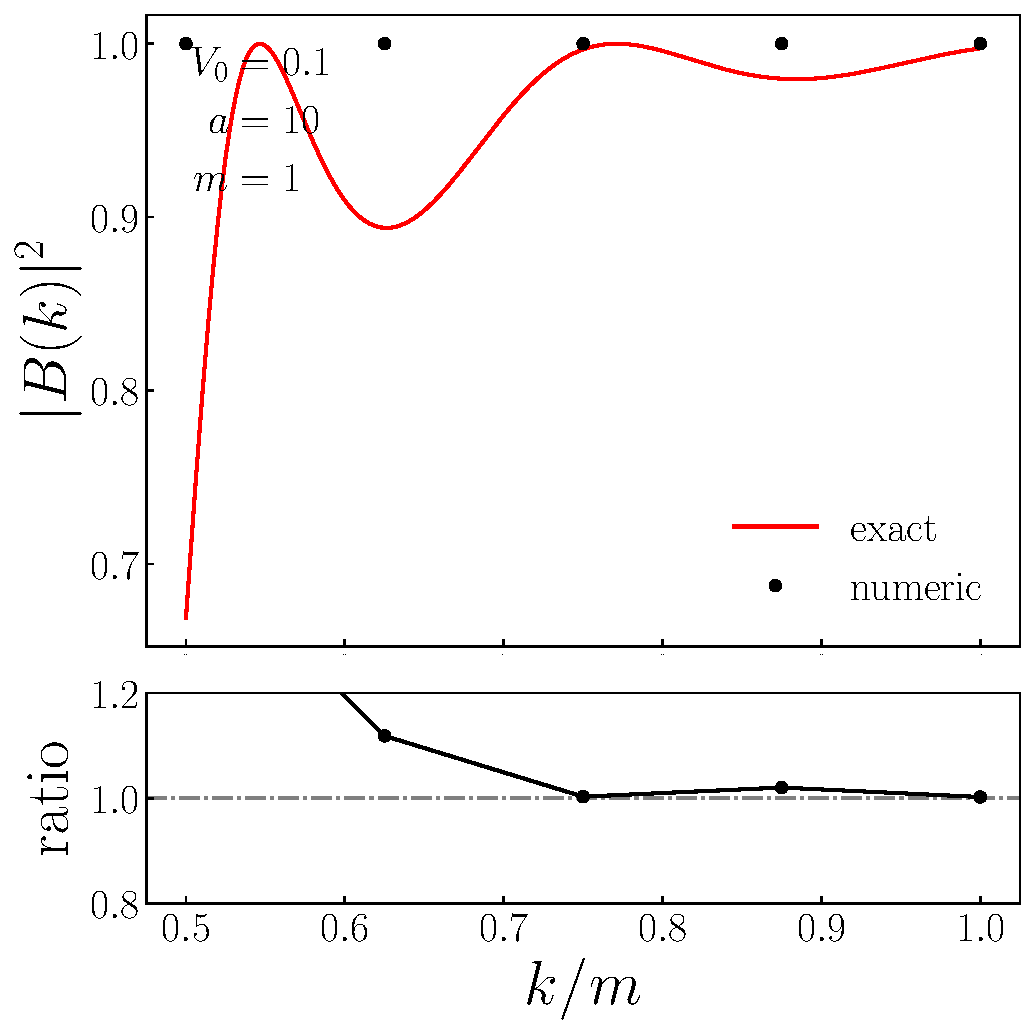
\includegraphics[width=0.7\linewidth]{square_barrier.pdf}
    \caption{\textbf{Top}: Comparison of the transmission probability predicted by Eq. (\ref{eq:square-barrier-Pt}) and by a dynamic numerical simulation of a wave packet. \textbf{Bottom}: Ratio of the numerical to the exact transmission probability for the settings shown in the top panel.}
    \label{fig:square-barrier}
\end{figure}



\section{Conclusions}
\label{sec:conclusions}

In this article, we have studied how to implement unitary time evolution of a wave function and the application of such time evolution to scattering in one dimension.
For our time evolution, we used the Backer-Campbell-Hausdorff formula to separate the free particle and potential pieces of the Hamiltonian such that over one time step the potential contributes as a phase shift, and the free-particle piece propagates the modes in space.
While the lattice simulation is time consuming and computationally intensive, it is clear that this method can be quite accurate given those resources and some fine-tuning to the parameters chosen for our simulations.
Additionally, the time evolution is readily generalizable to two or three dimensions.
Regarding the finite difference methods, it is perhaps worth studying further the shortcomings described here.
For example, one may explore whether renormalizing the wave function over time still yields faithful reconstructions of a free Gaussian wave packet as a first step, or perhaps one can implement a higher order formula for the time derivative, which suppresses the error in $\Delta t$ further.
Nevertheless, as a first step, the results presented in this article indicate a useful method for simulating quantum dynamics for localized potentials and some further steps to improve and expand the simulations shown here in order to produce realistic simulations of physical scattering processes.


\appendix

\section{Finite differences}
\label{app:finite-differences}

In Sec. \ref{ssec:numerical-techniques-for-unitary-time-evolution}, we alluded to the possibility of using finite difference formulas to determine our wave function at times $t > 0$ from some specified initial condition at $t = 0$.
Using a forward difference formula for the time derivative, the three-point formula for the second derivative, and rearranging, we obtain
\begin{align}
    \Psi_{n}^{(m + 1)} = \Psi_{n}^{(m)} + i \Delta t \Bigg( \frac{\Psi_{n-1}^{(m)} - 2 \Psi_{n}^{(m)} + \Psi_{n+1}^{(m)}}{2m \Delta x^2} - V_{n} \Psi_{n}^{(m)} \Bigg)
,\end{align}
as a discretized version of the Schr\"{o}dinger equation, where $\Psi_{n}^{(m)} = \Psi(x_n,t_{m})$, $x_{n} = x_0 + n \Delta x$, and $t_{m} = m \Delta t$.
Thus, we have a sequence defined by $\Psi_{n}^{(m)} = U^{m} \Psi_{n}^{(0)}$, where
\begin{align}
    U_{kn} = \delta_{kn} - i \Delta t H_{kn}
,\end{align}
where the discretized Hamiltonian
\begin{align}
    H_{kn} = -\frac{\delta_{k-1,n} - 2 \delta_{kn} + \delta_{k+1,n}}{2m \Delta x^2} + V_{k} \delta_{kn}
.\end{align}
This forms the basis of an explicit forward evolution scheme.
On the other hand, though, we could have used a backward difference formula for the time derivative and obtained $\Psi^{(m)} = U'^{-m} \Psi^{(0)}$, where $U'_{kn} = \delta_{kn} + i \Delta t H_{kn}$, which forms the basis of an implicit evolution scheme.

Because it is a fundamental tenet of quantum mechanics, we should ensure that the matrices being used to perform the time evolution are unitary, or at least approximately so.
For the explicit scheme, we check by direct multiplication:
\begin{align}
    U_{kn}^{\dagger} U_{nk'} &= ( \delta_{kn} + i \Delta t H_{kn}^{\dagger} ) ( \delta_{nk'} - i \Delta t H_{nk'} ) = \delta_{k k'} + i \Delta t ( H_{kk'}^{\dagger} - H_{kk'} ) + \Delta t^2 H_{kn}^{\dagger} H_{nk'} \nonumber \\
    &= \delta_{kk'} + \mathcal{O}(\Delta t^2)
.\end{align}
A similar formula holds for the implicit evolution scheme.
As mentioned above, herein lies a primary difficulty of implementing a finite difference method for the time evolution.
Although this formula indicates that our time evolution is essentially unitary over a single time step, over many steps the error accumulates to a significant and non-negligible level, and at such time, we violate probability conservation, which is essential to the interpretation of quantum mechanics and therefore our simulations.

\begin{figure}[tb]
    \centering
    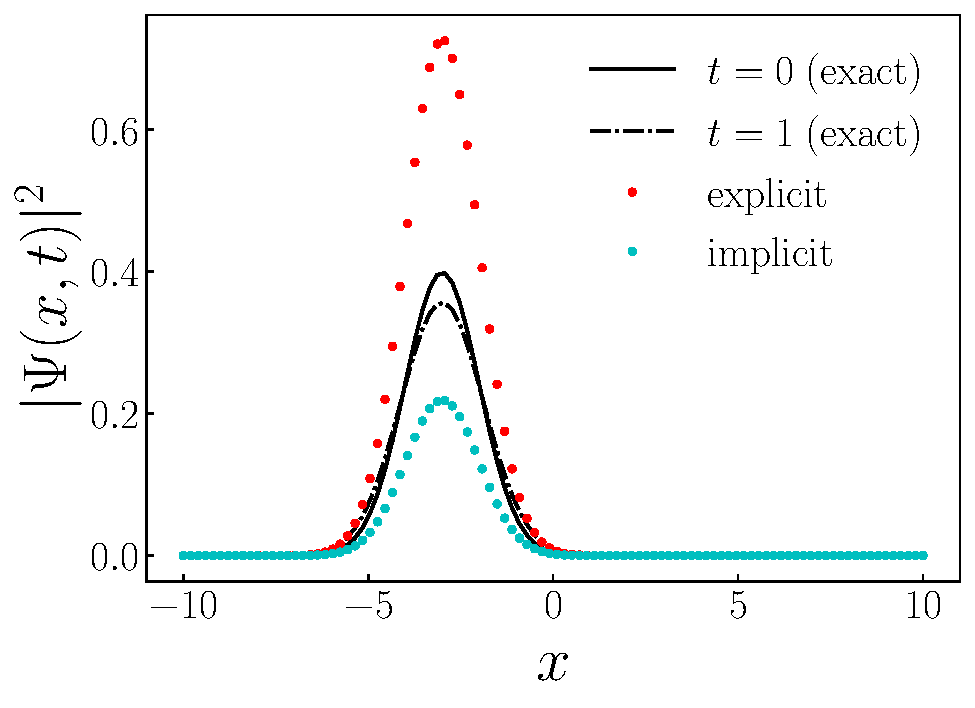
\includegraphics[width=0.7\linewidth]{finite_differences-evolution.pdf}
    \caption{Demonstration of the instability of the explicit and implicit finite difference methods for evolving a wave function, chosen to be a Gaussian, forward in time.}
    \label{fig:finite-differences-evolution}
\end{figure}


Another way of looking at the stability of our finite difference methods is the following.
Recall from linear algebra that a unitary operator admits a set of eigenvectors which form a basis of our space of interest.
While our finite matrices violate unitarity at the level of $\Delta t^2$, we can approximately for this argument approximately say that the eigenvectors of our finite matrices span our discretized space.
Let us denote the spectrum of $U$ by the set $\{ u_{n} \}$ and the corresponding set of eigenvectors by $\{ \phi^{(n)} \}$
Thus, any vector $\Psi$, which is analogous to our discretized wave-function, can be expanded as
\begin{align}
    \Psi = \sum_{n} c_{n} \phi^{(n)}
,\end{align}
where $c_{n} = \Psi^{\dagger} x^{(n)}$.
It follows then, that repeated action of $U$ on $\Psi$ yields
\begin{align}
    \Psi^{(k)} = U^{k} \Psi = \sum_{n} c_{n} u_{n}^{k} x^{(n)}
.\end{align}
Because of the discretization effects, our eigenvalues $u_{n}$ have approximately unit norm but not quite.
Thus, for large times (i.e. in the limit $k \rightarrow \infty$), we have
\begin{align}
    U^{k} \Psi \rightarrow c_{n_{\rm max}} u_{n_{\rm max}}^{k} \phi^{(n_{\rm max})}
,\end{align}
where $n_{\rm max} = {\rm argmax}(\{ |u_{n}| \})$.
Hence, if $|u_{n_{\rm max}}| > 1$ our solution explodes, and if $a_{\rm max} < 1$ our solution vanishes at large times.
Of course then, even the slightest bit of unitarity violation in our matrix evolution will scale with the number of time steps, which is demonstrated by Fig. \ref{fig:finite-differences-evolution}.
Although not shown here, the explicit evolution matrix has eigenvalues with norm larger than one, implying that $\Psi \rightarrow \infty$ in the limit $t \rightarrow \infty$, while on the other hand, the eigenvalues have norm less than one for the implicit evolution matrix and $\Psi \rightarrow 0$ in the limit $t \rightarrow \infty$, which is clearly observed in the figure.
While not explored here, it is perhaps possible that the error in the finite difference steps is predominately a scaling one.
If this is the case, then one could still employ the finite difference method and renormalize the wave function after some number of iterations.

    
\end{document}
